\section{Multiprocesinės operacinės sistemos modelis}

\subsection{Procesai}

Procesas - tai atskira vykdoma programa, kartu su esamomis registrų reikšmėmis ir savo kintamaisiais.
Kiekvienam procesui yra sukuriamas atskiras virtualus procesorius. Programa nuo proceso skiriasi tuo, kad procesas yra kokioje nors veikimo stadijoje esanti programa,
o programa - tam tikras baitų rinkinys. Proceso veikimo stadiją apibūdina proceso deskriptorius. Jame laikomi visi procesui reikalingi parametrai.\\

\subsubsection{Deskriptoriai}
Deskriptoriai yra dinaminiai objektai, kurie gali būsi sukurti ir sunaikinti sistemos veikimo metu. Procesus kuria procesai, todėl turi egzistuoti vienas pagrindinis procesas, 
kuriantis visus kitus.\\

Procesų deskriptoriai:
	\begin{itemize}
		\item PD - proceso vidinis vardas
		\item PID - proceso išorinis vardas
		\item PCPU - proceso būsena ir teisės
		\item PChild - proceso vaikų ID
		\item PParent - proceso tėvo ID
		\item PPriority - proceso prioritetas 0 - 100
		\item PRes - proceso sukurti resursai
		\item PRecRes - proceso kūrimo metu perduoti resursai
		\item PList - procesų sąrašas, kuriam priklauso procesas
	\end{itemize}

Procesus galima suskirstyti į:
	\begin{itemize}
		\item Vartotojiškus - vykdančius vartotojo programą
		\item Sisteminius - aptarnaujančius vartotojiškus.
	\end{itemize}

Procesas gauna procesorių tik tada, kai jam netrūksta jokio kito resurso ir tampa vykdomu. Tokioje būsenoje procesas išlieka tol, kol sistemoje neįvyksta pertraukimas 
arba einamasis procesas nepaprašo kokio nors resurso. Jei procesas nereikalauja jokio resurso, iš jo gali būti atimtas procesorius, nes per ilgai dirbo.\\
Procesų būsenos:
	\begin{itemize}
		\item Vykdomas - turi procesorių
		\item Blokuotas - prašo resurso (išskyrus procesorių)
		\item Pasiruošęs - vienintelis trūkstamas resursas yra procesorius
		\item Sustabdytas - kito proceso sustabdytas procesas
	\end{itemize}

Diagrama, vaizduojanti, kaip procesas gali pakliūti i tam tikrą būseną ir iš jos išeiti:

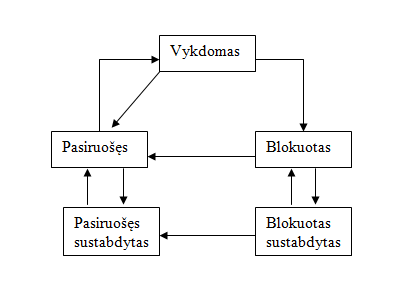
\includegraphics{processDiagram.png}

	\begin{itemize}
		\item Vykdomas procesas blokuojasi jam prašant ir negavus resurso.
		\item Vykdomas procesas tampa pasiruošusiu atėmus iš jo procesorių dėl kokios nors priežasties
		\item Blokuotas procesas tampa pasiruošusiu, kai yra suteikiamas reikalingas resursas.
		\item Pasiruošę procesai varžosi dėl procesoriaus. Gavęs procesorių procesas tampa vykdomu.
		\item Procesas gali tapti sustabdytu blokuotu, jei einamasis procesas jį sustabdo, kai jis jau ir taip jau yra blokuotas
		\item Procesas tampa blokuotu iš blokuoto sustabdyto, jei einamasis procesas nuima būseną sustabdytas.
		\item Procesas gali tapti pasiruošusiu sustabdytu, jei einamasis procesas jį sustabdo, kai jis yra pasiruošęs.
		\item Procesas tampa pasiruošusiu iš pasiruošusio sustabdyto, jei einamasis procesas nuima būseną sustabdytas.
		\item Procesas tampa pasiruošusiu iš blokuoto sustabdyto, jei procesui yra suteikiamas jam reikalingas resursas.
	\end{itemize}

\subsubsection{Procesų planuotojas}
Procesų planuotojo paskirtis - atimti procesorių iš proceso, peržvelgti pasiruošusių procesų sąrašą, išrinkti iš jo tinkamiausią procesą ir jam perduoti procesorių.
Planuotojas turi įgyvendinti šias užduotis:
	\begin{itemize}
		\item Kiekvienas procesas pagrįstą laiko tarpa turi turėti procesorių
		\item Laikyti procesorių užimtą netoli 100%
		\item Nuveiktų darbų skaičius turi būti maksimalus
		\item Vartotojai atsakymo turi laukti mažiausiai laiko
	\end{itemize}

Planuotojas yra prioritetais besiremiantis algoritmas. Proceso prioritetas - jo vykdymo svarba skalėje nuo 1 iki 100. Procesas su aukštesniu prioritetu yra arčiau procesų sąrašo pradžios.
Kuo aukščiau yra procesas, tuo daugiau jis turi galimybių tapti vykdomu (jei pasiruošęs) arba pasiruošusiu (jei blokuotas). Planuotojas iškviečiamas norint pakeisti einamąjį procesą kitu.

Diagrama, vaizduojanti planuotojo veiksmų seką:

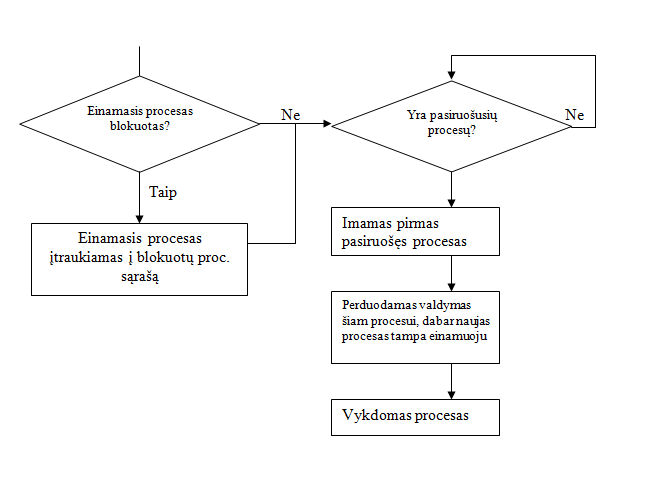
\includegraphics{processPlanner.png}

\subsubsection{Procesų primityvai}
Procesų primityvų paskirtis - pateikti vienodą ir paprastą vartotojo sąsają darbui su procesais. Kiekvieno primityvo programos gale yra kviečiamas planuotojas. Yra 4 primityvai:
	\begin{itemize}
		\item Kurti procesą - primityvui perduodama nuoroda į jo tėvą, jo pradinė būsena, prioritetas, perduodamų elementų sąrašas ir išorinis vardas.
			Tada procesas yra registruojamas bendrame procesų sąraše, tėvo sūnų sąraše, skaičiuojamas vidinis identifikacijos numeris.
		\item Naikinti procesą - pradedama naikinti proceso sukurtus resursus ir vaikus. Vėliau procesas panaikinamas iš tėvo procesų sąrašo. Po to iš bendro procesų sąrašo, galiausiai
			naikinami visi jam perduoti resursai ir proceso deskriptorius yra sunaikinamas.
		\item Stabdyti procesą - proceso būsena iš blokuotos keičiama į blokuotą-sustabdytą arba į pasiruošusią-sustabdytą. Einamasis procesas tampa pasiruošusiu-sustabdytu.
		\item Aktyvuoti procesą - keičiama proceso būsena iš blokuotos-sustabdyto į blokuotą arba pasiruošusios-sustabdytos į pasiruošusią.
	\end{itemize}


